\iffalse
\let\negmedspace\undefined
\let\negthickspace\undefined
\documentclass[journal,12pt,onecolumn]{IEEEtran}
\usepackage{cite}
\usepackage{amsmath,amssymb,amsfonts,amsthm}
\usepackage{algorithmic}
\usepackage{graphicx}
\usepackage{textcomp}
\usepackage{xcolor}
\usepackage{txfonts}
\usepackage{listings}
\usepackage{enumitem}
\usepackage{mathtools}
\usepackage{gensymb}
\usepackage{comment}
\usepackage[breaklinks=true]{hyperref}
\usepackage{tkz-euclide} 
\usepackage{listings}
\usepackage{gvv}                                        
\def\inputGnumericTable{}                                 
\usepackage[latin1]{inputenc}                                
\usepackage{color}                                            
\usepackage{array}                                            
\usepackage{longtable}                                       
\usepackage{calc}                                             
\usepackage{multirow}                                         
\usepackage{hhline}                                           
\usepackage{ifthen}                                           
\usepackage{lscape}

\newtheorem{theorem}{Theorem}[section]
\newtheorem{problem}{Problem}
\newtheorem{proposition}{Proposition}[section]
\newtheorem{lemma}{Lemma}[section]
\newtheorem{corollary}[theorem]{Corollary}
\newtheorem{example}{Example}[section]
\newtheorem{definition}[problem]{Definition}
\newcommand{\BEQA}{\begin{eqnarray}}
 \newcommand{\EEQA}{\end{eqnarray}}
\newcommand{\define}{\stackrel{\triangle}{=}}
\theoremstyle{remark}
\newtheorem{rem}{Remark}
\begin{document}
 \bibliographystyle{IEEEtran}
 \vspace{3cm}
 \title{\textbf{11.14-4}}
 \author{EE23BTECH11048-Ponugumati Venkata Chanakya$^{*}$% <-this % stops a space
 }
 \maketitle

 \bigskip
 \renewcommand{\thefigure}{\theenumi}
 \renewcommand{\thetable}{\theenumi}
 \textbf{QUESTION:}
 Which of the following functions of time represent (a) simple harmonic, (b) periodic
 but not simple harmonic, and (c) non-periodic motion? Give period for each case of periodic motion ($\omega$ is any positive constant):\\
 \begin{enumerate}
 \item $\sin\brak{\omega t}-\cos\brak{\omega t}$\\
 \item $\sin^3\brak{\omega t}$\\
 \item $3\cos\brak{\frac{\pi}{4}- 2\omega t}$\\
 \item $\cos\brak{\omega t}+\cos\brak{3\omega t}+\cos\brak{5\omega t}$\\
 \item \text{exp}\brak{-\omega^2 t^2}\\
 \item $1+\omega t+\omega^2 t^2$\\
  \end{enumerate}
 \solution:\\
\fi
 \begin{enumerate}
   \item Periodic function:
   \begin{align}
x(t+T) = x(t) \quad \forall x \in \mathbb{R}
\end{align}
 where min $T$ s.t $T>0$ is time period\\
 \\
   \item SHM:\\
    For a function to be in shm it must satisfy 
    \begin{align}
   \frac{d^2 x(t)}{dt^2} = - (2\pi f_0)^2 x(t)
      \end{align}
      \end{enumerate}
   \begin{enumerate}
   \begin{table}[!ht]
    \centering
        
      \begin{tabular}{|c|c|c|} 
      \hline
\textbf{Variable}& \textbf{Description}& formula\\\hline
         $x(t)$&  Displacemen wrt mean position&none\\\hline
          $\omega$&Angular frequncy&$2\pi f$\\\hline
          $T$& Time period &$\frac{1}{f}$ \\ \hline
          $\phi$& phase angle &none \\ \hline
    \end{tabular}

    \caption{input parameters}
    \label{tab:}
\end{table}
\item $\sin(2\pi f t)- \cos(2\pi f t)$\\
The function can be rewritten as:
 \begin{align}
  &= \sin(2\pi f t) - \sin\brak{\frac{\pi}{2} - 2\pi f t}\\
  &=2 \cos\brak{\frac{\pi}{4}} \sin\brak{2\pi f t - \frac{\pi}{4}}\\
  &=\sqrt{2}\sin\brak{2\pi f t - \frac{\pi}{4}}\\
  \frac{d^2(\sin(2\pi f t)- \cos(2\pi f t))}{dt^2}&=-(2\pi f)^2(\sin(2\pi f t)- \cos(2\pi f t))\\
     \frac{d^2 x(t)}{dt^2} &= - (2\pi f)^2 x(t)\\
     \end{align}
     
 $\therefore$ SHM, $T$ is $\frac{1}{f}$and $\phi$ is $\brak{\frac{-\pi}{4}}$ or $\brak{\frac{7\pi}{4}}$\\
 
 \begin{align}
 \sin\brak{2\pi f\brak{t+\frac{1}{f}}}- \cos\brak{2\pi f\brak{t+\frac{1}{f}}}&=\sin(2\pi f t)- \cos(2\pi f t)
 \end{align}
Graph of function is shown in (\figref{fig:11.14.4.2})
\\
    \item[(3)] $3\cos\brak{\frac{\pi}{4}-4\pi f t}$\\

This function can be rewritten as\\ 
 \begin{align}
  &=3\cos\brak{4\pi f t-\frac{\pi}{4}}\\
  \frac{d^2\brak{3\cos\brak{\frac{\pi}{4}-4\pi f t}}}{dt^2}&=-3(4\pi f)^2\brak{\cos\frac{\pi}{4}-4\pi f t}\\
  \frac{d^2 x(t)}{dt^2} &= - (4\pi f)^2 x(t)
 \end{align}
 $\therefore$  SHM, $T$ is $\frac{1}{2f}$  and  $\phi$ is $\brak{\frac{-\pi}{4}} or \brak{\frac{7\pi}{4}} $\\
 \begin{align}
 3\cos\brak{\frac{\pi}{4}-4\pi f \brak{t+\frac{1}{2f}}}=3\cos\brak{\frac{\pi}{4}-4\pi f t}\\
 \end{align}
 Graph of function is shown in (\figref{fig:11.14.4.3})
 \\

 \item[(4)]  $\cos(2\pi f t)+\cos(6\pi  f t)+\cos(10\pi  f t)$\\

This function can be rewritten as\\ 
 \begin{align}
  &=\cos(2\pi f t)+\cos(10\pi  f t)+\cos(6\pi  f t)\\
  &=2\cos\brak{\frac{2\pi f t+10\pi f t}{2}}\cos\brak{\frac{10\pi  f t-2\pi f t}{2}} +\cos(6\pi f t)\\
  &=2\cos(6\pi  f t) \cos(2\pi f t)+\cos(6\pi  f t)\\
  &=\cos(6\pi  f t) (1+2\cos(2\pi f t))\\
     \frac{d^2{\cos(2\pi f t)+\cos(6\pi  f t)+\cos(10\pi  f t)}}{dt^2}&=(2\pi f)^2\cos(2\pi f t)+(6\pi f)^2\cos(6\pi  f t)+(10\pi f)^2\cos(10\pi  f t)\\
      \frac{d^2 x(t)}{dt^2} &\neq - (2\pi f)^2 x(t)
 \end{align}
 Period of $\cos(6\pi  f t)$ is $\frac{1}{3f}$\\ 
 Period of $1+2\cos(2\pi f t)$ is $\frac{1}{f}$\\ 
 Lcm is $\frac{1}{f}$\\
 $\therefore$  SHM,$T$ is $\frac{1}{f}$\\
 \begin{align}   
 \cos\brak{2\pi f \brak{t+\frac{1}{f}}}+\cos\brak{6\pi  f \brak{t+\frac{1}{f}}}+\cos\brak{10\pi  f \brak{t+\frac{1}{f}}}=\cos(2\pi f t)+\cos(6\pi  f t)+\cos(10\pi  f t)
 \end{align}
 Graph of function is shown in (\figref{fig:11.14.4.4})
 \\

 \item[(5)]  $\text{exp}\brak{-(2\pi f)^2 t^2}$\\

       \begin{align}
     \text{As } T\to\infty\\
    \text{exp}\brak{-(2\pi f)^2 t^2}\to \infty\\ 
    \frac{d^2(\text{exp}\brak{-(2\pi f)^2 t^2}))}{dt^2}&=2(2\pi ft)^2\text{exp}\brak{-(2\pi f)^2 t^2}+2(2\pi ft)^4\text{exp}\brak{-(2\pi f)^2 t^2}\\
    \frac{d^2 x(t)}{dt^2} &\neq - (2\pi f)^2 x(t)
       \end{align}
    $\therefore$  This never repeats and non periodic\\
    Graph of function is shown in (\figref{fig:11.14.4.5})
    \\
    
 \item[(6)] $1+2\pi f t+(2\pi f)^2t^2$\\

 \begin{align}
  \text{As } T\to\infty\\
  1+2\pi f t+(2\pi f)^2t^2  \to \infty\\
   \frac{d^2(1+2\pi f t+(2\pi f)^2t^2)}{dt^2}&=2(2\pi f)^2\\
   \frac{d^2 x(t)}{dt^2} &\neq - (2\pi f)^2 x(t)
 \end{align}
  $\therefore$ This never repeats and non periodic\\ 
 Graph of function is shown in (\figref{fig:11.14.4.6})
 \begin{flushleft}
  \begin{table}[h]
   \def\arraystretch{1.5}:
   \caption{Summary}
   \begin{tabular}{|l|c|c|c|c|c|c|}
  \hline
  &\textbf{Function}&\textbf{Periodic } &\textbf{Simple harmonic motion}&\textbf{Non Periodic}& \textbf{T}& $\phi$ \\\hline
  (a) & $\sin(2\pi ft)-\cos(2\pi ft)$ & Yes & Yes & No & $\frac{1}{f }$&\brak{\frac{-\pi}{4}} \\\hline
  (b) & $\sin^3(2\pi ft)$  & Yes & No & No & $\frac{1}{f}$&$-$\\\hline
  (c) & $3\cos\brak{\frac{\pi}{4}-4\pi ft}$ & Yes & Yes & No & $\frac{1}{2f}$& \brak{\frac{-\pi}{4}}\\\hline
  (d) & $\cos(2\pi ft)+\cos(6\pi ft)+\cos(10\pi ft)$ & Yes & No & No & $\frac{}{f}$&$-$\\\hline
  (e) & $\text{exp}\brak{-(2\pi ft)^2}$ & No & No & Yes & $-$&$-$ \\\hline
  (f) &$ 1+(2\pi f)  t+(2\pi f)  ^2t^2$ & No & No & Yes & $-$ &$-$\\\hline
 \end{tabular}


  \end{table}
 \end{flushleft}
 
\end{enumerate}
 \renewcommand{\thefigure}{\theenumi}
 \renewcommand{\thetable}{\theenumi}
 
 
 \begin{figure}[h!]
    \centering
    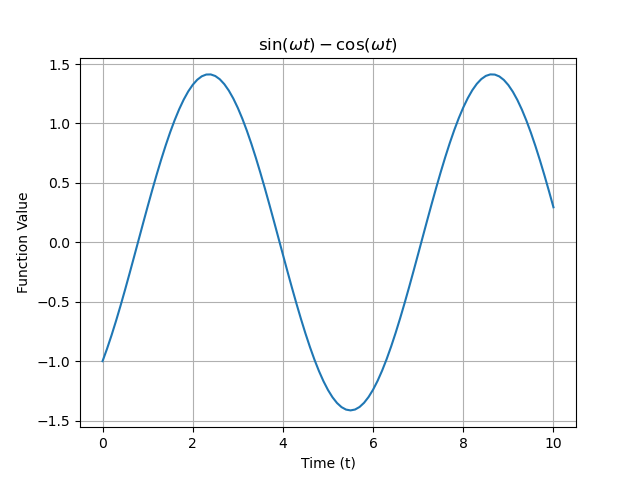
\includegraphics[width=\columnwidth]{ncert-physics/11/14/4/figs/11.14.4 f1.png}
    \caption{$\sin(2\pi f t)- \cos(2\pi f t)$}
    \label{fig:11.14.4.1}
\end{figure}
 \begin{figure}[h!]
    \centering
    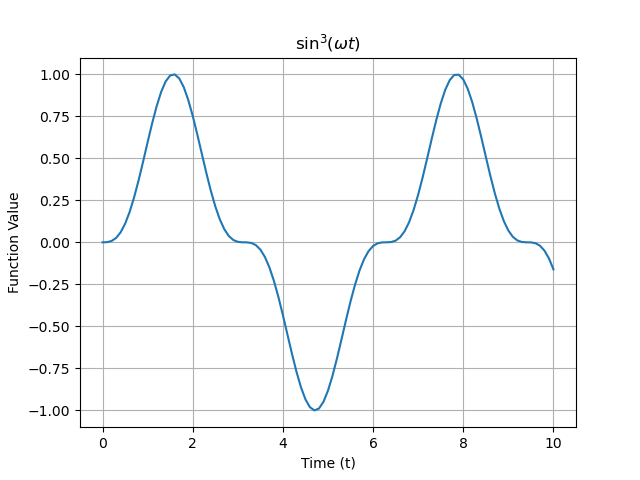
\includegraphics[width=\columnwidth]{ncert-physics/11/14/4/figs/11.14.4 f2.png}
    \caption{$\sin^3(2\pi f t)$}
    \label{fig:11.14.4.2}
\end{figure}
\newpage
\begin{figure}[h!]
    \centering
    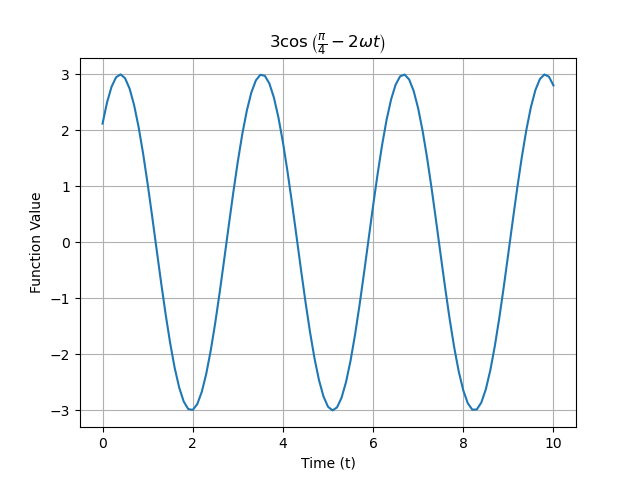
\includegraphics[width=\columnwidth]{ncert-physics/11/14/4/figs/11.14.4 f3.png}
    \caption{$3\cos\brak{\frac{\pi}{4}- 4\pi f t}$}
    \label{fig:11.14.4.3}
\end{figure}
\begin{figure}[h!]
    \centering
    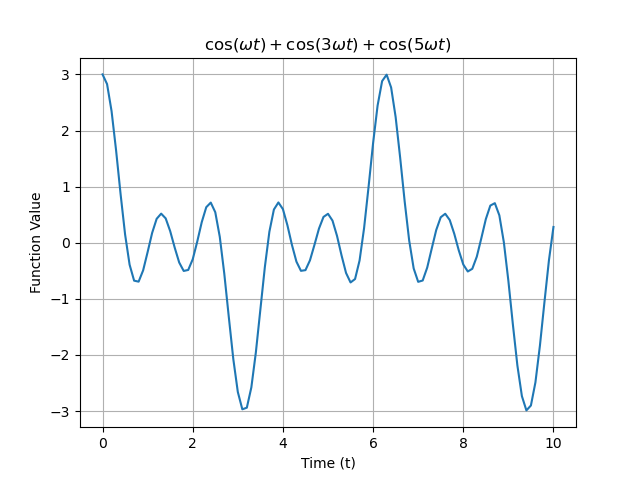
\includegraphics[width=\columnwidth]{ncert-physics/11/14/4/figs/11.14.4 f4.png}
    \caption{$\cos(2\pi f t)+\cos(6\pi  f t)+\cos(10\pi  f t)$}
    \label{fig:11.14.4.4}
\end{figure}
\begin{figure}[h!]
    \centering
    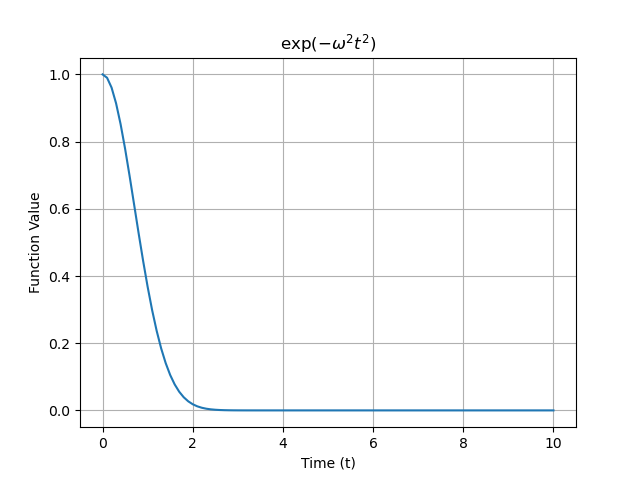
\includegraphics[width=\columnwidth]{ncert-physics/11/14/4/figs/11.14.4 f5.png}
    \caption{$exp^{\brak{-(2\pi ft)^2}}$}
    \label{fig:11.14.4.5}
\end{figure}
\begin{figure}[h!]
    \centering
    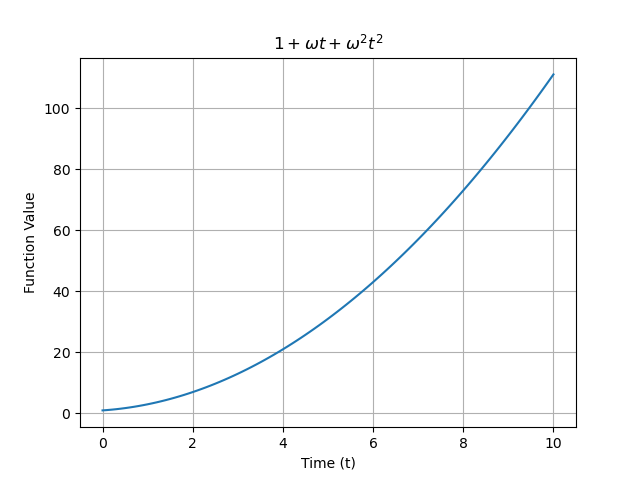
\includegraphics[width=\columnwidth]{ncert-physics/11/14/4/figs/11.14.4 f6.png}
    \caption{$1+2\pi f t+(2\pi f t)^2$}
    \label{fig:11.14.4.6}
\end{figure}
%\end{document}
